%!TEX root = document.tex
\section*{Opgave A}
\begin{enumerate}
  \item
  Jeg benytter følgende propositionsvariable:
  \begin{itemize}
    \item $P_r$: P er ridder
    \item $Q_r$: Q er ridder
  \end{itemize}
  Hvis P ikke er en ridder må P være en bonde, da der kun findes to typer af mennesker på øen. Altså kan jeg udtrykke at P er en bonde ved $\lnot P_r$. Ligeledes kan jeg udtrykke at Q er en bonde ved $\lnot Q_r$.

  For at bestemme hvad P og Q er, ser jeg først på Ps svar på spørgsmålet. Man må kunne udtrykke at mindst én af dem er en bonde ved:
  \begin{equation}
    \label{A1:udsagn}
    \lnot P_r \lor \lnot Q_r
  \end{equation}
  Hvis \eqref{A1:udsagn} er sandt må $P_r$ være sandt, da P i så fald har talt sandt og derved ikke kan være en bonde. Hvis \eqref{A1:udsagn} er falsk må $P_r$ være falsk, da P i så fald har løjet og derved ikke kan være en ridder.

  Ligeledes må \eqref{A1:udsagn} være falsk hvis $P_r$ er falsk, og sandt hvis $P_r$ er sand.

  Altså må der være tale om en biimplikation, og situationen kan beskrives ved:
  \begin{equation}
    \label{A1:situation}
    P_r \leftrightarrow \lnot P_r \lor \lnot Q_r
  \end{equation}

  Jeg kan undersøge hvilke værdier der vil gøre \eqref{A1:situation} sand vha. tableau-metoden:
  \begin{equation*}
    \begin{tikzpicture}[level distance=8mm,sibling distance=50mm]
      \node {$P_r \leftrightarrow \lnot P_r \lor \lnot Q_r : \T\ \checkmark$}
      child {
        node {$P_r : \T$}
        child {
          node {$\lnot P_r \lor \lnot Q_r : \T\ \checkmark$}
          child {
            node {$\lnot P_r : \T\ \checkmark$}
            child {
              node {$P_r : \F$}
              \closed
            }
          }
          child {
            node {$\lnot Q_r : \T\ \checkmark$}
            child {
              node {$Q_r : \F$}
              \open
            }
          }
        }
      }
      child {
        node {$P_r : \F$}
        child {
          node {$\lnot P_r \lor \lnot Q_r : \F\ \checkmark$}
          child {
            node {$\lnot P_r : \F\ \checkmark$}
            child {
              node {$\lnot Q_r : \F$}
              child {
                node {$P_r : \T$}
                \closed
              }
            }
          }
        }
      };
    \end{tikzpicture}
  \end{equation*}

  Det ses at der kun en én åben, mættet gren, hvor $P_r$ er sand og $Q_r$ er falsk.

  Altså er P en ridder og Q en bonde.

  \item
  Jeg benytter følgende propositionsvariable:
  \begin{itemize}
    \item $A_r$: A er ridder
    \item $B_r$: B er ridder
  \end{itemize}

  Svaret A giver kan udtrykkes ved:
  \begin{equation}
    \lnot B_r \rightarrow \lnot A_r
  \end{equation}

  Ligesom før kan situationen beskrives ved en biimplikation mellem A og svaret A gav:
  \begin{equation}
    \label{A2:situation}
    B_r \leftrightarrow \left( \lnot B_r \rightarrow \lnot A_r \right)
  \end{equation}

  Undersøger hvilke værdier der opfylder \eqref{A2:situation} vha. tableau-metoden:
  \begin{equation*}
    \begin{tikzpicture}[level distance=8mm,sibling distance=50mm]
      \node {$A_r \leftrightarrow \left( \lnot B_r \rightarrow \lnot A_r \right) : \T\ \checkmark$}
      child {
        node {$A_r : \T$}
        child {
          node {$\lnot B_r \rightarrow \lnot A_r : \T\ \checkmark$}
          child {
            node {$\lnot B_r : \F\ \checkmark$}
            child {
              node {$B_r : \T$}
              \open
            }
          }
          child {
            node {$\lnot A_r : \T$}
            child {
              node {$A_r : \F$}
              \closed
            }
          }
        }
      }
      child {
        node {$A_r : \F$}
        child {
          node {$\lnot B_r \rightarrow \lnot A_r : \F\ \checkmark$}
          child {
            node {$\lnot B_r : \T$}
            child {
              node {$\lnot A_r : \F\ \checkmark$}
              child {
                node {$A_r : \T$}
                \closed
              }
            }
          }
        }
      };
    \end{tikzpicture}
  \end{equation*}

  Det ses at der kun er én åben, mættet gren, hvor $A_r$ er sand og $B_r$ er sand.

  Altså er både A og B riddere.

  \item
  Jeg benytter følgende propositionsvariable:
  \begin{itemize}
    \item $C_r$: C er ridder
    \item $C_k$: C er kannibal
    \item $D_r$: D er ridder
    \item $D_k$: D er kannibal
    \item $E_r$: E er ridder
    \item $E_k$: E er kannibal
  \end{itemize}

  Der er nu tre udsagn. C's formodede svar, at kun én af dem er en ridder, kan udtrykkes ved:
  \begin{equation}
    \label{A3:Csvar}
    \left( C_r \land \left( \lnot D_r \land \lnot E_r \right) \right) \lor \left( \lnot C_r \land \left( D_r \land \lnot E_r \right) \right) \lor \left( \lnot C_r \land \left( \lnot D_r \land E_r \right) \right)
  \end{equation}

  E siger at D er en bonde og at E ikke er en kannibal. Det kan udtrykkes ved:
  \begin{equation}
    \label{A3:Esvar}
    \lnot D_r \land \lnot E_k
  \end{equation}

  D siger at D ikke er en kannibal, hvilket kan udtrykkes ved:
  \begin{equation}
    \label{A3:Dsvar}
    \lnot D_k
  \end{equation}

  Ligesom før kan situationen beskrives vha. biimplikationer. \eqref{A3:Csvar} afhænger først og fremmest af om C er en ridder (og derved taler sandt). Situationen for C kan da udtrykkes ved:
  \begin{equation}
    \label{A3:Csituation}
    \begin{split}
      C_r \leftrightarrow & \left( C_r \land \left( \lnot D_r \land \lnot E_r \right) \right) \lor\\
      & \left( \lnot C_r \land \left( D_r \land \lnot E_r \right) \right) \lor \left( \lnot C_r \land \left( \lnot D_r \land E_r \right) \right)
    \end{split}
  \end{equation}

  Da D stod for oversættelsen fra det C sagde, må \eqref{A3:Csituation} afhænge af hvorvidt D er en ridder. Det D selv sagde afhænger selvfølgelig også af om D er en ridder. Altså er C's situation en del af D's situation, og derved kan \eqref{A3:Csituation} og \eqref{A3:Dsvar} samles i et udtryk for D's situation:
  \begin{equation}
    \begin{split}
      D_r \leftrightarrow \lnot D_k \land ( C_r \leftrightarrow & \left( C_r \land \left( \lnot D_r \land \lnot E_r \right) \right) \lor\\
      & \left( \lnot C_r \land \left( D_r \land \lnot E_r \right) \right) \lor \left( \lnot C_r \land \left( \lnot D_r \land E_r \right) \right) )
    \end{split}
  \end{equation}

  E's situation kan udtrykkes ved:
  \begin{equation}
    E_r \leftrightarrow \lnot D_r \land \lnot E_k
  \end{equation}

  Ved at samle situationerne for D, som indeholder situationen for C, og E kan jeg få et udtryk for den samlede situation ved:
  \begin{equation}
    \begin{split}
      \left( E_r \leftrightarrow & \lnot D_r \land \lnot E_k\right) \land (
      D_r \leftrightarrow \lnot D_k \land ( C_r \leftrightarrow \left( C_r \land \left( \lnot D_r \land \lnot E_r \right) \right) \lor\\
      & \left( \lnot C_r \land \left( D_r \land \lnot E_r \right) \right) \lor \left( \lnot C_r \land \left( \lnot D_r \land E_r \right) \right) ))
    \end{split}
  \end{equation}

  Tableau-metoden:
  \begin{equation*}
    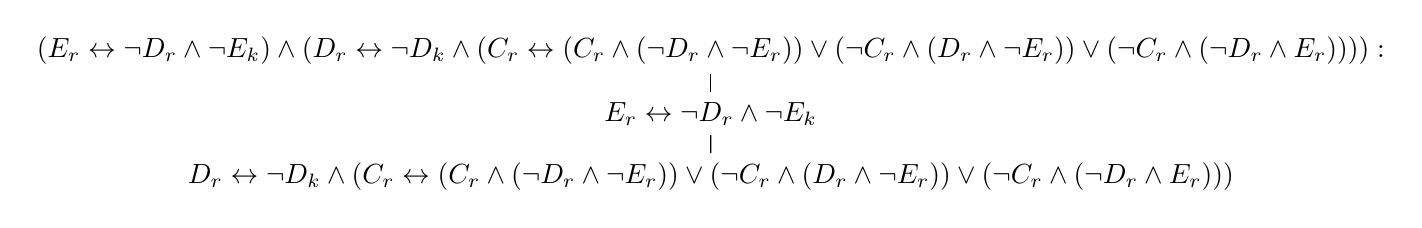
\begin{tikzpicture}[level distance=8mm,sibling distance=50mm]
      \node {$\left( E_r \leftrightarrow \lnot D_r \land \lnot E_k\right) \land (
      D_r \leftrightarrow \lnot D_k \land ( C_r \leftrightarrow \left( C_r \land \left( \lnot D_r \land \lnot E_r \right) \right) \lor
      \left( \lnot C_r \land \left( D_r \land \lnot E_r \right) \right) \lor \left( \lnot C_r \land \left( \lnot D_r \land E_r \right) \right) )) : \T$}
      child {
        node {$E_r \leftrightarrow \lnot D_r \land \lnot E_k$}
        child {
          node {$D_r \leftrightarrow \lnot D_k \land ( C_r \leftrightarrow \left( C_r \land \left( \lnot D_r \land \lnot E_r \right) \right) \lor
                \left( \lnot C_r \land \left( D_r \land \lnot E_r \right) \right) \lor \left( \lnot C_r \land \left( \lnot D_r \land E_r \right) \right) )$}
        }
      };
    \end{tikzpicture}
  \end{equation*}
\end{enumerate}